\chapter{Methodology}

\vspace{-1cm}

This chapter shows the process of designing, testing and troubleshooting tools and equipment, construction and wiring procedure.

Now that the design is in place, the purchase of material will follow, then the construction of the device and lastly the performance,
functionality, and reliability will be tested.

\section{System Design}
\begin{figure}[ht]
  \centering \begin{tikzpicture}
    \node[anchor=north west] (battery) at (0, -0.3) {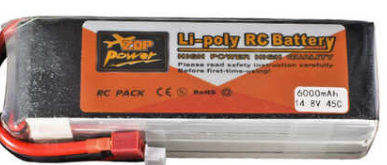
\includegraphics[width=3cm]{assets/battery.png}};
    \node[anchor=north west] (converter) at (5, 0) {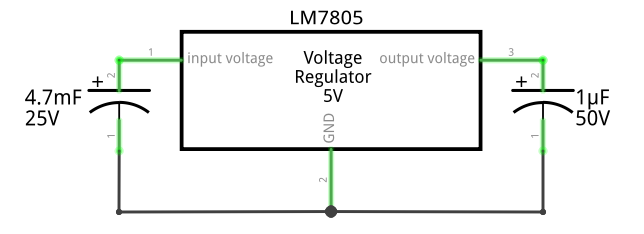
\includegraphics[width=5cm]{assets/converter.png}};
    \node[anchor=north west] (esp32) at (6, -3.5) {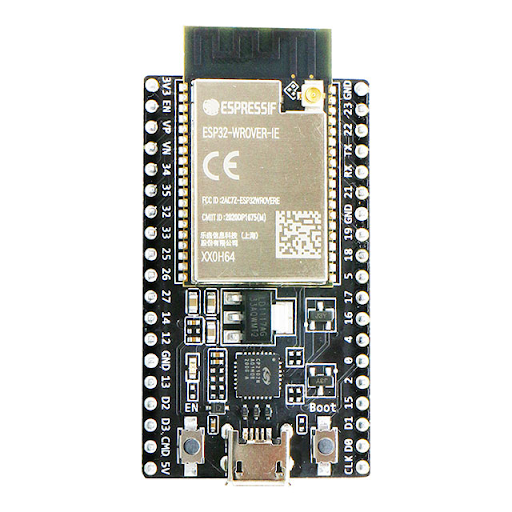
\includegraphics[width=3cm]{assets/esp-32.png}};
    \node[anchor=north west] (magnetometer) at (12, -0.5) {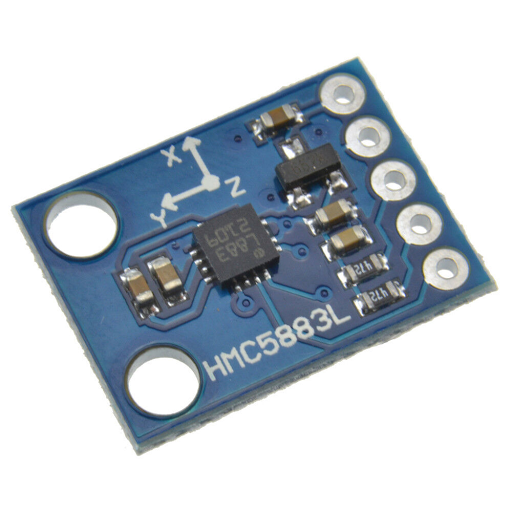
\includegraphics[width=3cm]{assets/magnetometer.png}};
    \node[anchor=north west] (gps) at (12, -6) {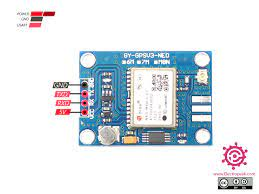
\includegraphics[width=3cm]{assets/gps_module.png}};
    \node[anchor=north west] (esc) at (0, -3.5) {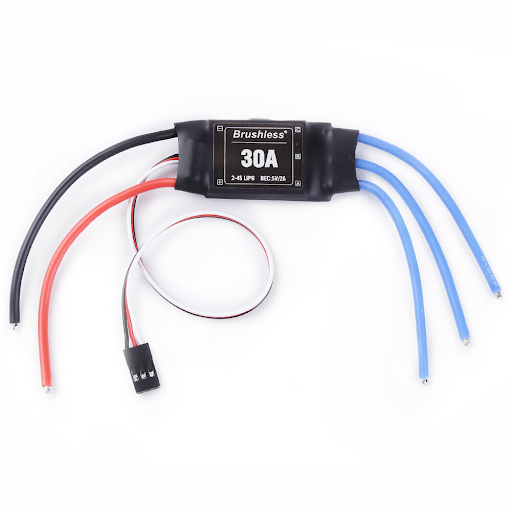
\includegraphics[width=3cm]{assets/esc.png}};
    \node[anchor=north west] (motor) at (3, -8) {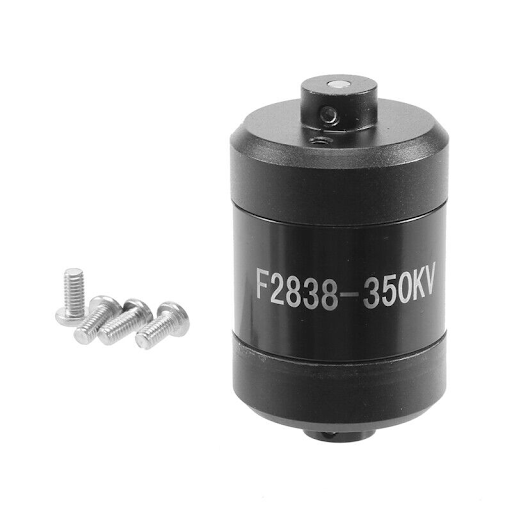
\includegraphics[width=3cm]{assets/motor.png}};
    \node[anchor=north west] (propeller) at (9, -8.2) {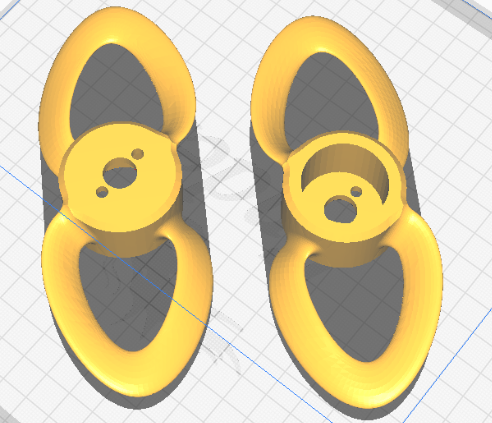
\includegraphics[width=3cm]{assets/propellers.png}};

    \draw[ ->, line width = 1mm, black!70] (battery) to (converter);
    \draw[ ->, line width = 1mm, black!70] (battery) to (esc);
    \draw[ ->, line width = 1mm, black!70] (esp32) to (esc);
    \draw[ <->, line width = 1mm, black!70] (esc) |- (motor);
    \draw[ ->, line width = 1mm, black!70] (motor) to (propeller);
    \draw[ ->, line width = 1mm, black!70] (converter) to (esp32);
    \draw[ <->, line width = 1mm, black!70] (esp32.east) + (0, 0.3) -| (magnetometer.south);
    \draw[ <->, line width = 1mm, black!70] (esp32.east) + (0, -0.2) -| (gps.north);

    % \path[ ->, line width = 1mm, black!70] (esp32.east) + (0, 1) edge [bend left] (magnetometer);
    % \path[ <-, line width = 1mm, black!70] (esp32.east) + (0, 0.5) edge [bend right] (magnetometer.west);
    % \path[ ->, line width = 1mm, black!70] (esp32.east) + (0, -0.5) edge [bend right] (gps);
    % \path[ <-, line width = 1mm, black!70] (esp32.east) + (0, 0) edge [bend left] (gps.west);


  \end{tikzpicture}
  \caption{System Design}
  \label{fig:SystemDesign}
\end{figure}

\pagebreak

% \section{Flowchart}
% \begin{figure}[ht]
% \centering \begin{tikzpicture}
%   [
%   RECT/.style={rectangle, rounded corners, draw=black!60, fill=white!0, very thick, minimum width = 20mm, minimum height = 10mm, align = center},
%   ROUNDEDRECT/.style={rounded rectangle, draw=black!60, fill=white!0, very thick, minimum width = 20mm, minimum height = 10mm},
%   DIAMOND/.style={diamond, draw=black!60, fill=white!0, very thick, minimum width = 10mm, minimum height = 10mm, align = center, aspect = 2, },
%   ]

%   \node[ROUNDEDRECT] (start) {Start};
%   \node[RECT] (switchOn) [below = of start] {Switch on};
%   \node[RECT] (esp32Boot) [right = of switchOn] {ESP-32 boots};
%   \node[RECT] (waitForUserInput) [right = of esp32Boot] {Waiting for user \\ input coordinates};
%   \node[RECT] (coordinatesSupplied) [below = of waitForUserInput] {Coordinates Supplied};
%   \node[RECT] (detectsLocationData) [left = of coordinatesSupplied] {GPS \& magnetometer \\ detects location data};
%   \node[RECT] (droneMoves) [left = of detectsLocationData] {Drone moves to \\ supplied coordinates};
%   \node[RECT] (confirmLoc) [below = of droneMoves] {GPS \& magnetometer \\ confirms location data};
%   \node[] (dummyNode) [below = of detectsLocationData] {};
%   \node[DIAMOND] (doesLocMatch) [below = of dummyNode] {Does drone location match \\ with supplied coordinates?};
%   \node[RECT] (terminate) [below = of doesLocMatch] {Drone terminated};
%   \node[ROUNDEDRECT] (end) [right = of terminate] {End};

%   \draw[ ->, line width = 1mm, black!70] (start.south) to node[] {} (switchOn.north);
%   \draw[ ->, line width = 1mm, black!70] (switchOn.east) to node[] {} (esp32Boot.west);
%   \draw[ ->, line width = 1mm, black!70] (esp32Boot.east) to node[] {} (waitForUserInput.west);
%   \draw[ ->, line width = 1mm, black!70] (waitForUserInput.south) to node[] {} (coordinatesSupplied.north);
%   \draw[ ->, line width = 1mm, black!70] (coordinatesSupplied.west) to node[] {} (detectsLocationData.east);
%   \draw[ ->, line width = 1mm, black!70] (detectsLocationData.west) to node[] {} (droneMoves.east);
%   \draw[ ->, line width = 1mm, black!70] (droneMoves.south) to node[] {} (confirmLoc.north);
%   \draw[ ->, line width = 1mm, black!70] (confirmLoc.south) to node[] {} (doesLocMatch.west);
%   \draw[ ->, line width = 1mm, black!70] (doesLocMatch.north) to node[left] {NO} (detectsLocationData.south);
%   \draw[ ->, line width = 1mm, black!70] (doesLocMatch.south) to node[left] {YES} (terminate.north);
%   \draw[ ->, line width = 1mm, black!70] (terminate.east) to node[] {} (end.west);
% \end{tikzpicture}
% \caption{Flowchart}
% \label{fig:Flowchart}
% \end{figure}

\section{Flowchart}
\begin{figure}[ht]
  \centering \begin{tikzpicture}
    [
      RECT/.style={rectangle, rounded corners, draw=black!60, fill=white!0, very thick, minimum width = 20mm, minimum height = 10mm, align = center},
      ROUNDEDRECT/.style={rounded rectangle, draw=black!60, fill=white!0, very thick, minimum width = 20mm, minimum height = 10mm},
      DIAMOND/.style={diamond, draw=black!60, fill=white!0, very thick, minimum width = 10mm, minimum height = 10mm, align = center, aspect = 3, },
    ]

    \node[ROUNDEDRECT] (start) {Start};
    \node[RECT] (switchOn) [right = of start] {Switch on};
    \node[RECT] (waitForUserInput) [below right = of switchOn] {Waiting for \\ user to provide \\ target coordinates};
    \node[RECT] (waitingForSensor) [below left = of switchOn] {Waiting for GPS and \\ magnetometer modules to \\ process  location and heading};
    \node[DIAMOND] (isUserInputValid) [below = of waitForUserInput] {Is user input \\ valid?};
    \node[DIAMOND] (isSensorDataValid) [below = of waitingForSensor] {Is sensor data \\ valid?};
    \node[RECT] (compute) [below = 5.5cm of switchOn] {Compute distance and \\ bearing to target};
    \node[RECT] (move) [below = of compute] {Drone turns and \\ moves to target};
    \node[DIAMOND] (distance) [below = of move] {Is the distance between \\ the drone and the target within the \\ uncertainty threshold?};
    \node[RECT] (terminate) [below = of distance] {Drone terminated};
    \node[ROUNDEDRECT] (end) [right = of terminate] {End};

    \draw[ ->, line width = 1mm, black!70] (start) to (switchOn);
    \draw[ ->, line width = 1mm, black!70] (switchOn.south) + (3mm, 0) |- (waitForUserInput.west);
    \draw[ ->, line width = 1mm, black!70] (switchOn.south) + (-3mm, 0) |- (waitingForSensor.east);
    \draw[ ->, line width = 1mm, black!70] (waitForUserInput) to (isUserInputValid);
    \draw[ ->, line width = 1mm, black!70] (waitingForSensor) to (isSensorDataValid);
    \draw[ ->, line width = 1mm, black!70] (isSensorDataValid.south)  |- node[below] {Yes} (compute.west);
    \draw[ ->, line width = 1mm, black!70] (isUserInputValid.south) |- node[below] {Yes} (compute.east);
    \draw[ ->, line width = 1mm, black!70] (compute) to (move);
    \draw[ ->, line width = 1mm, black!70] (move) to (distance);
    \draw[ ->, line width = 1mm, black!70] (distance) to node[left] {Yes} (terminate);
    \draw[ ->, line width = 1mm, black!70] (terminate) to (end);
    \draw[ ->, line width = 1mm, black!70] (isSensorDataValid) + (-3, 0) node[below] {No} |- (waitingForSensor.west);
    \draw[ -, line width = 1mm, black!70] (waitingForSensor) + (-3, 0) |- (isSensorDataValid.west);
    \draw[ ->, line width = 1mm, black!70] (isUserInputValid) + (3, 0) node[below] {No} |- (waitForUserInput.east);
    \draw[ -, line width = 1mm, black!70] (waitForUserInput) + (3, 0) |- (isUserInputValid.east);
    \draw[ ->, line width = 1mm, black!70] (distance) + (-6, 0) node[below] {No} |- (move.west);
    \draw[ -, line width = 1mm, black!70] (move) + (-6,0) |- (distance.west);

  \end{tikzpicture}
  \caption{Flowchart}
  \label{fig:Flowchart}
\end{figure}

\pagebreak
\section{Navigation algorithm}
\begin{enumerate}
  \item  Get target location \tLoc from the user

        \tLoc is acquired from the user by specifying its geo-coordinates in the \emph{Latitude-Longitude} format. Latitude values denote the angular distance relative
        to the equator, with positive values indicating locations north of the equator and negative values indicating locations south of the equator. Similarly, Longitude values
        represent the angular distance east or west of the Prime Meridian, with positive values corresponding to western locations and negative values signifying eastern locations.
        \emph{Both Latitude and Longitude should be specified as decimal degrees.}

  \item  Get current location \cLoc and current heading \cHeading from GPS and magnetometer modules

        \cLoc is acquired from the Global Positioning System (GPS) module. The module transmits NMEA sentences (refer to Section X.X todo for a detailed
        explanation) to the ESP32 microcontroller.  Of these sentences, the GPGLL sentence is specifically processed to extract the latitude, north/south (N/S) indicator, longitude,
        east/west (E/W) indicator, and validity status.  The latitude and longitude values are converted from the degrees-minutes-decimal minutes format (dddmm.mmmm)
        to decimal degrees for further calculations.  Subsequently, the N/S and E/W indicators are used to determine the correct sign (positive or negative) for the extracted
        latitude and longitude values.

        In contrast, \cHeading, is calculated based on the \emph X and \emph Y values obtained from the magnetometer module.
        This value represents the device's orientation relative to magnetic north. The calculation of \cHeading requires the declination angle \decAngle which is itself derived from the
        longitude component of the current location, \cLoc. The declination correction accounts for the difference between magnetic north and true geographic north.  This correction is 
        applied to the magnetic heading, denoted by \cHeading which is am azimuth value between 0 and 359 degrees, to obtain a value that represents the device's orientation relative to 
        true north. A specific function is used during this correction process to ensure the resulting value remains within the 0-359 degree range and avoids overflow errors.

          \large $$ \text{let } \lambda_c = \text{longitude component of } X_c $$
          \large $$ \delta = (\underbrace{0.015}_{\mathclap {\text{constant used to approximate angle of declination}}} * \lambda_c) + 1 $$
          \large $$ \theta_c = \atantwo(y, x) + \frac{180}{\pi} + \delta $$


  \item Get the difference between between longitude and latitude components of \cLoc and \tLoc

        \small   $$ \text{let } \lambda_c = \text{longitude component of } X_c $$
        \small   $$ \text{let } \lambda_t = \text{longitude component of } X_t $$
        \small   $$ \text{let } \phi_c = \text{latitude component of } X_c $$
        \small   $$ \text{let } \phi_t = \text{latitude component of } X_t $$

        \large  $$ \lambda = \lambda_c - \lambda_t $$
        \large $$ \phi = \phi_c - \phi_t $$
  
  \item Get bearing \bearing to target
\end{enumerate}